\documentclass[12pt, a4paper, oneside, openright, titlepage]{book}
\usepackage[utf8]{inputenc}
\raggedbottom
%%%%%%%%%%%%%%%%% Book Formatting Comments:

%%%%%%%%%%%%%%%%%%%%%%%%%%%%%%%%%%%%% for Part

%%%%%%%%%%%%%%%%%%%%%% for chapter

%%%%%%%%%%%%%%%%%%%% for section




%%%%%% PACKAGES %%%%%%%
\usepackage{hyperref}
\hypersetup{
    colorlinks,
    citecolor=black,
    filecolor=black,
    linkcolor=black,
    urlcolor=black
}
\usepackage{amsmath} % Math display options
\usepackage{amssymb} % Math symbols
%\usepackage{amsfonts} % Math fonts
%\usepackage{amsthm}
\usepackage{mathtools} % General math tools
\usepackage{array} % Allows you to write arrays
\usepackage{empheq} % For boxing equations
% \usepackage{mathabx}
% \usepackage{mathrsfs}
\usepackage{nameref}
\usepackage{wrapfig}

\usepackage{soul}
\usepackage[normalem]{ulem}

\usepackage{txfonts}
\usepackage{cancel}
\usepackage[toc, page]{appendix}
\usepackage{titletoc,tocloft}
\setlength{\cftchapindent}{1em}
\setlength{\cftsecindent}{2em}
\setlength{\cftsubsecindent}{3em}
%\setlength{\cftsubsubsecindent}{4em}
\usepackage{titlesec}

%\titleformat{\section}
%  {\normalfont\fontsize{25}{15}\bfseries}{\thesection}%{1em}{}
%\titleformat{\section}
%  {\normalfont\fontsize{20}{15}\bfseries}%{\thesubsection}{1em}{}
%\setcounter{secnumdepth}{1}  
  
  

%\newcommand\numberthis{\refstepcounter{equation}\tag{\theequation}} % For equation labelling
\usepackage[framemethod=tikz]{mdframed}

\usepackage{tikz} % For drawing commutative diagrams
\usetikzlibrary{cd}
\usetikzlibrary{calc}
\tikzset{every picture/.style={line width=0.75pt}} %set default line width to 0.75p

\usepackage{datetime}
\usepackage[margin=1.5in]{geometry}
\setlength{\parskip}{1em}
\usepackage{makeidx}         % allows index generation
\usepackage{graphicx}       % standard LaTeX graphics tool
\usepackage{multicol}        % used for the two-column index
\usepackage[bottom]{footmisc}% places footnotes at page bottom

\usepackage{newtxtext}       % 
\usepackage{newtxmath}       % selects Times Roman as basic font
\usepackage{float}
\usepackage{fancyhdr}
\setlength{\headheight}{15pt} 
\pagestyle{fancy}
\lhead[\leftmark]{}
\rhead[]{\leftmark}

%\usepackage{enumitem}

\usepackage{url}
\allowdisplaybreaks

%%%%%% ENVIRONMENTS %%%
\definecolor{purp}{rgb}{0.29, 0, 0.51}
\definecolor{bloo}{rgb}{0, 0.13, 0.80}



%%\newtheoremstyle{note}% hnamei
%{3pt}% hSpace above
%{3pt}% hSpace belowi
%{}% hBody fonti
%{}% hIndent amounti
%{\itshape}% hTheorem head fonti
%{:}% hPunctuation after theorem headi
%{.5em}% hSpace after theorem headi
%{}% hTheorem head spec (can be left empty, meaning ‘normal’)i





% %%%%%%%%%%%%% THEOREM DEFINITIONS

\spnewtheorem{axiom}{Axiom}[chapter]{\bfseries}{\itshape}


\spnewtheorem{construction}{Construction}[chapter]{\bfseries}{\itshape}

\spnewtheorem{props}{Properties}[chapter]{\bfseries}{\itshape}


\renewcommand{\qedsymbol}{$\blacksquare$}


\numberwithin{equation}{section}

\newenvironment{qest}{
    \begin{center}
        \em
    }
    {
    \end{center}
    }

%%%%%% MACROS %%%%%%%%%
%% New Commands
\newcommand{\ip}[1]{\langle#1\rangle} %%% Inner product
\newcommand{\abs}[1]{\lvert#1\rvert} %%% Modulus
\newcommand\diag{\operatorname{diag}} %%% diag matrix
\newcommand\tr{\mbox{tr}\.} %%% trace
\newcommand\C{\mathbb C} %%% Complex numbers
\newcommand\R{\mathbb R} %%% Real numbers
\newcommand\Z{\mathbb Z} %%% Integers
\newcommand\Q{\mathbb Q} %%% Rationals
\newcommand\N{\mathbb N} %%% Naturals
\newcommand\F{\mathbb F} %%% An arbitrary field
\newcommand\ste{\operatorname{St}} %%% Steinberg Representation
\newcommand\GL{\mathbf{GL}} %%% General Linear group
\newcommand\SL{\mathbf{SL}} %%% Special linear group
\newcommand\gl{\mathfrak{gl}} %%% General linear algebra
\newcommand\G{\mathbf{G}} %%% connected reductive group
\newcommand\g{\mathfrak{g}} %%% Lie algebra of G
\newcommand\Hbf{\mathbf{H}} %%% Theta fixed points of G
\newcommand\X{\mathbf{X}} %%% Symmetric space X
\newcommand{\catname}[1]{\normalfont\textbf{#1}}
\newcommand{\Set}{\catname{Set}} %%% Category set
\newcommand{\Grp}{\catname{Grp}} %%% Category group
\newcommand{\Rmod}{\catname{R-Mod}} %%% Category r-modules
\newcommand{\Mon}{\catname{Mon}} %%% Category monoid
\newcommand{\Ring}{\catname{Ring}} %%% Category ring
\newcommand{\Topp}{\catname{Top}} %%% Category Topological spaces
\newcommand{\Vect}{\catname{Vect}_{k}} %%% category vector spaces'
\newcommand\Hom{\mathbf{Hom}} %%% Arrows

\newcommand{\map}[2]{\begin{array}{c} #1 \\ #2 \end{array}}

\newcommand{\Emph}[1]{\textbf{\ul{\emph{#1}}}}




%% Math operators
\DeclareMathOperator{\ran}{Im} %%% image
\DeclareMathOperator{\aut}{Aut} %%% Automorphisms
\DeclareMathOperator{\spn}{span} %%% span
\DeclareMathOperator{\ann}{Ann} %%% annihilator
\DeclareMathOperator{\rank}{rank} %%% Rank
\DeclareMathOperator{\ch}{char} %%% characteristic
\DeclareMathOperator{\ev}{\bf{ev}} %%% evaluation
\DeclareMathOperator{\sgn}{sign} %%% sign
\DeclareMathOperator{\id}{Id} %%% identity
\DeclareMathOperator{\supp}{Supp} %%% support
\DeclareMathOperator{\inn}{Inn} %%% Inner aut
\DeclareMathOperator{\en}{End} %%% Endomorphisms
\DeclareMathOperator{\sym}{Sym} %%% Group of symmetries


%% Diagram Environments
\iffalse
\begin{center}
    \begin{tikzpicture}[baseline= (a).base]
        \node[scale=1] (a) at (0,0){
          \begin{tikzcd}
           
          \end{tikzcd}
        };
    \end{tikzpicture}
\end{center}
\fi




\newdateformat{monthdayyeardate}{%
    \monthname[\THEMONTH]~\THEDAY, \THEYEAR}
%%%%%%%%%%%%%%%%%%%%%%%

\usetikzlibrary{decorations.pathmorphing}
%%%%%% BEGIN %%%%%%%%%%


\begin{document}

%%%%%% TITLE PAGE %%%%%

\begin{titlepage}
    \centering
    \scshape
    \vspace*{\baselineskip}
    \rule{\textwidth}{1.6pt}\vspace*{-\baselineskip}\vspace*{2pt}
    \rule{\textwidth}{0.4pt}
    
    \vspace{0.75\baselineskip}
    
    {\LARGE Category Theory: A Viewpoint of Math}
    
    \vspace{0.75\baselineskip}
    
    \rule{\textwidth}{0.4pt}\vspace*{-\baselineskip}\vspace{3.2pt}
    \rule{\textwidth}{1.6pt}
    
    \vspace{2\baselineskip}
    Category Theory \\
    \vspace*{3\baselineskip}
    \monthdayyeardate\today \\
    \vspace*{5.0\baselineskip}
    
    {\scshape\Large Elijah Thompson, \\ Physics and Math Honors\\}
    
    \vspace{1.0\baselineskip}
    \textit{Solo Pursuit of Learning}
    \vfill
    \enlargethispage{1in}
    \begin{figure}[b!]
    \makebox[\textwidth]{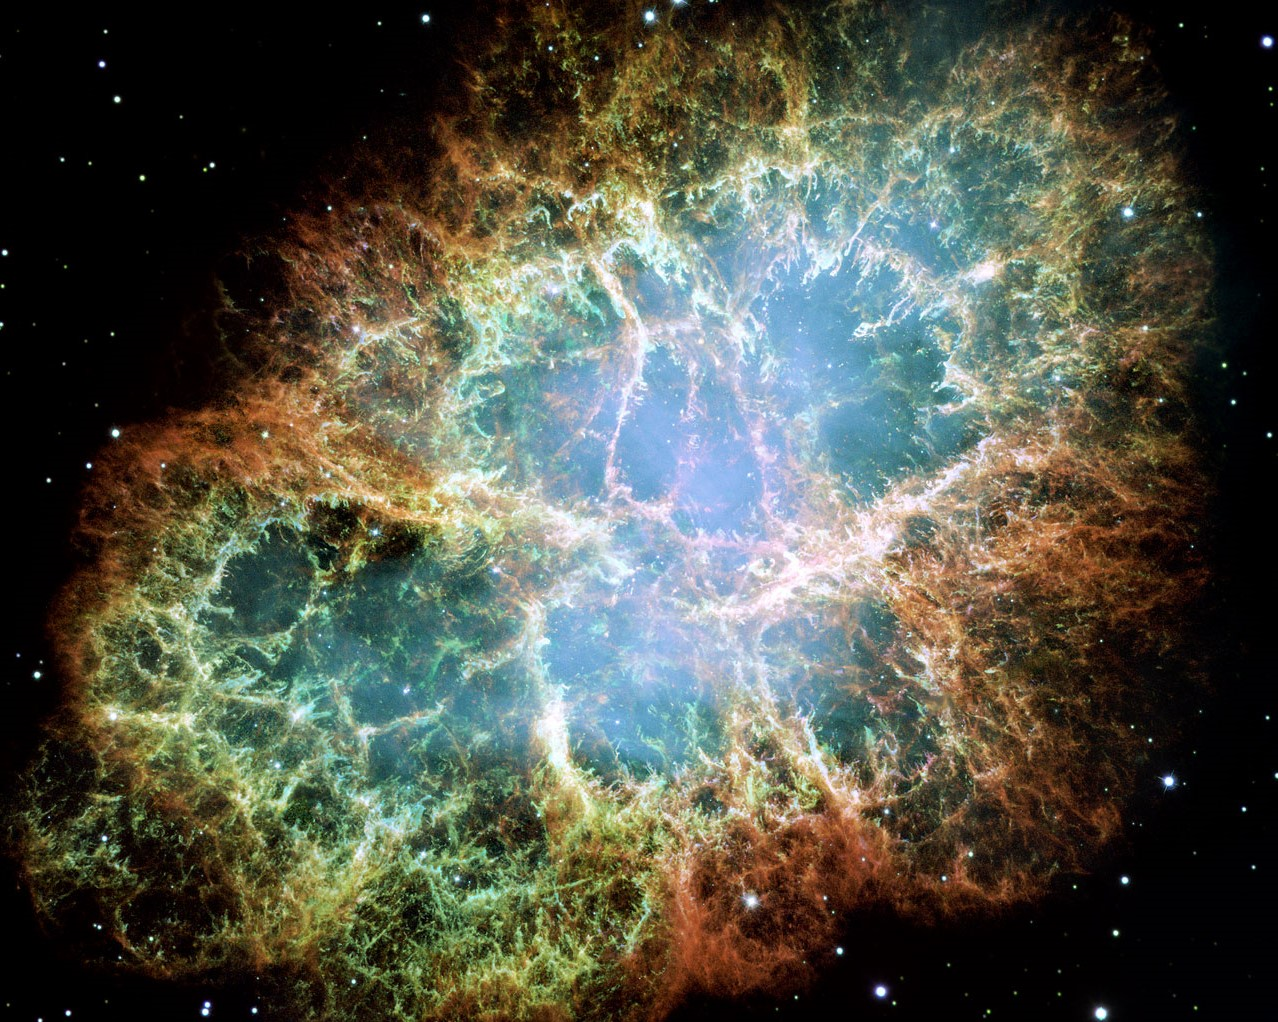
\includegraphics[width=\paperwidth, height =10cm]{../../Crab.jpg}}
    \end{figure}
\end{titlepage}

%%%%%%%%%%%%%%%%%%%%%%%
\tableofcontents





%%%%%%%%%%%%%%%%%%%%%%% - P1.Chapter 1
\chapter{Categories and Fundamental Examples}

\section{Category Definitions}

\begin{defn}
    A \Emph{category} $\catname{C}$ is given by the following data: \begin{enumerate}
        \item a class $\catname{Ob}(\catname{C})$ of objects of $\catname{C}$
        \item a family $\Hom_{\catname{C}}$ associating with each pair $A, B \in \catname{C}$ a class $\Hom_{\catname{C}}(A,B)$ of morphisms from $A$ to $B$
    \end{enumerate}
    so that:
    \begin{enumerate}
        \item For a morphism $f \in \Hom_{\catname{C}}(A,B)$, we say that $A$ is the \Emph{domain} object of $f$ and \Emph{codomain} object of $f$, and we write $f:A\rightarrow B$. 
        \item For each object $A$ of $\catname{C}$ there is a designated \Emph{identity morphism} $\id_A \in \Hom_{\catname{C}}(A,A)$ (i.e. $\id_A:A\rightarrow A$).
        \item For all $A, B, C \in \catname{Ob}(\catname{C})$ a mapping \begin{equation*}
                \circ: \Hom_{\catname{C}}(B,C)\times \Hom_{\catname{C}}(A,B) \rightarrow \Hom_{\catname{C}}(A,C)
        \end{equation*}
            called composition exists, and is defined such that for all $f \in \Hom_{\catname{C}}(A,B)$ and $g \in \Hom_{\catname{C}}(B,C)$, the following diagram commutes:
				\begin{center}
					\begin{tikzpicture}[baseline= (a).base]
						\node[scale=1] (a) at (0,0){
						  \begin{tikzcd}
						  		& B \ar[dr, "g"] & \\
                    			A \ar[ur, "f"] \ar[rr, "g\circ f"] & & C
						  \end{tikzcd}
						};
					\end{tikzpicture}
				\end{center} 
                such that $g\circ f \in \Hom_{\catname{C}}(A,C)$ is called the \Emph{composite morphism}.
    \end{enumerate}
    This data is subject to the following axioms: \begin{enumerate}
        \item For any objects $A$ and $B$ and morphism $f:A\rightarrow B$, the composites $\id_B\circ f$ and $f\circ \id_A$ are equal to $f$.
        \item For any composable triple of morphisms $f:A\rightarrow B$, $g:B\rightarrow C$, and $h:C\rightarrow D$, the composites $h\circ(g\circ f)$ and $(h\circ g)\circ f$ are equal. In particular, the following diagram commutes:
            \begin{center}
               \tikzset{every picture/.style={line width=0.75pt}} %set default line width to 0.75pt        

\begin{tikzpicture}[x=0.75pt,y=0.75pt,yscale=-1,xscale=1]
%uncomment if require: \path (0,300); %set diagram left start at 0, and has height of 300


% Text Node
\draw (125,142.4) node [anchor=north west][inner sep=0.75pt]    {$A$};
% Text Node
\draw (127,53.4) node [anchor=north west][inner sep=0.75pt]    {$B$};
% Text Node
\draw (246,53.4) node [anchor=north west][inner sep=0.75pt]    {$C$};
% Text Node
\draw (245,142.4) node [anchor=north west][inner sep=0.75pt]    {$D$};
% Text Node
\draw (121,102.4) node [anchor=north west][inner sep=0.75pt]  [font=\tiny]  {$f$};
% Text Node
\draw (191,49.4) node [anchor=north west][inner sep=0.75pt]  [font=\tiny]  {$g$};
% Text Node
\draw (257,102.4) node [anchor=north west][inner sep=0.75pt]  [font=\tiny]  {$h$};
% Text Node
\draw (173,83.4) node [anchor=north west][inner sep=0.75pt]  [font=\tiny]  {$h\circ g$};
% Text Node
\draw (152,113.4) node [anchor=north west][inner sep=0.75pt]  [font=\tiny]  {$g\circ f$};
% Text Node
\draw (148,153.4) node [anchor=north west][inner sep=0.75pt]  [font=\tiny]  {$h\circ ( g\circ f) \ =\ ( h\circ g) \circ f$};
% Connection
\draw    (132.13,138) -- (132.85,74) ;
\draw [shift={(132.87,72)}, rotate = 450.64] [color={rgb, 255:red, 0; green, 0; blue, 0 }  ][line width=0.75]    (10.93,-3.29) .. controls (6.95,-1.4) and (3.31,-0.3) .. (0,0) .. controls (3.31,0.3) and (6.95,1.4) .. (10.93,3.29)   ;
% Connection
\draw    (142,60.5) -- (241,60.5) ;
\draw [shift={(243,60.5)}, rotate = 180] [color={rgb, 255:red, 0; green, 0; blue, 0 }  ][line width=0.75]    (10.93,-3.29) .. controls (6.95,-1.4) and (3.31,-0.3) .. (0,0) .. controls (3.31,0.3) and (6.95,1.4) .. (10.93,3.29)   ;
% Connection
\draw    (252.44,72) -- (252.08,136) ;
\draw [shift={(252.06,138)}, rotate = 270.32] [color={rgb, 255:red, 0; green, 0; blue, 0 }  ][line width=0.75]    (10.93,-3.29) .. controls (6.95,-1.4) and (3.31,-0.3) .. (0,0) .. controls (3.31,0.3) and (6.95,1.4) .. (10.93,3.29)   ;
% Connection
\draw    (142,142.11) -- (183.65,111.35)(199.74,99.47) -- (241.39,68.7) ;
\draw [shift={(243,67.52)}, rotate = 503.55] [color={rgb, 255:red, 0; green, 0; blue, 0 }  ][line width=0.75]    (10.93,-3.29) .. controls (6.95,-1.4) and (3.31,-0.3) .. (0,0) .. controls (3.31,0.3) and (6.95,1.4) .. (10.93,3.29)   ;
% Connection
\draw    (142,67.23) -- (240.4,140.82) ;
\draw [shift={(242,142.02)}, rotate = 216.79] [color={rgb, 255:red, 0; green, 0; blue, 0 }  ][line width=0.75]    (10.93,-3.29) .. controls (6.95,-1.4) and (3.31,-0.3) .. (0,0) .. controls (3.31,0.3) and (6.95,1.4) .. (10.93,3.29)   ;
% Connection
\draw    (142,149.5) -- (240,149.5) ;
\draw [shift={(242,149.5)}, rotate = 180] [color={rgb, 255:red, 0; green, 0; blue, 0 }  ][line width=0.75]    (10.93,-3.29) .. controls (6.95,-1.4) and (3.31,-0.3) .. (0,0) .. controls (3.31,0.3) and (6.95,1.4) .. (10.93,3.29)   ;

\end{tikzpicture} 
            \end{center}
    \end{enumerate}
    That is, the composition law is associative and unital with the identity morphisms serving as two-sided identites.
\end{defn}

\begin{rmk}
    The objects of a category are in bijective correspondence with the identity morphisms, which are uniquely determined by the property that they serve as two-sided identities with composition. Thus, we can define a category as a collection of morphisms with a partially defined composition operation that has certain special morphisms which are used to recognize composable pairs and which serve as two-sided identites. 
\end{rmk}


\begin{eg}
    \leavevmode
    \begin{enumerate}
        \item $\Set$ is the category with sets as its objections and set-theoretic functions, with specified domain and codomain, as its morphisms
        \item $\Topp$ is the category with topological spaces as its objects and continuous functions as its morphisms.
        \item $\Set_*$ ($\Topp_*$) are the categories with sets (spaces) with a specified basepoint as objects and basepoint preserving (continuous) functions as morphisms. Note that a \Emph{basepoint} is a distinguished point in the set (space).
        \item $\Grp$ is the category with groups homomorphisms as morphisms. The categories $\Ring$ of associative and unital rings and ring homomorphisms and $\catname{Field}$ of fields and field homomorphisms are defined similarly.
        \item For a fixed unital but not necessarily commutative ring $R$, $\Rmod$ is the category of left $R$-modules and $R$-module homomorphisms. Th:is category is denoted by $\Vect$ when the ring happends to be a field $k$ and abbreviated as $\catname{Ab}$ (for abelian groups) in the case of $\catname{Mod}_{\Z}$, as a $\Z$-module is precisely an abelian group.
        \item $\catname{Graph}$ is the category with graphs as objects and graph morphisms (functions carrying vertices to vertices and edges to edges, preserving incidence relations) as morphisms. In the variant $\catname{DirGraph}$, objects are directed graphs, whose edges are now depicted as arrows, and morphisms are directed graph morphisms, which preserve sources and targets.
        \item $\catname{Man}$ is the category with smooth (i.e. infinitely differentiable) manifolds as objects and smooth maps as morphisms.
        \item $\catname{Meas}$ is the category with measurable spaces as objects and measurable functions as morphisms. 
        \item $\catname{Poset}$ is the category with partially ordered sets as objects and order-preserving functions as morphisms.
        \item $\catname{Ch}_R$ is the category with chain complexes of $R$-modules as objects and chain homomorphisms as morphisms.
            \begin{defn}
                A \Emph{chain complex} $C_*$ is a collection $(C_n)_{n \in \Z}$ of $R$-modules equipped with $R$-module homomorphisms $d:C_n\rightarrow C_{n-1}$, called \Emph{boundary homomorphisms}, with the property that $d^2 = 0$, i.e., the composite of any two boundary maps is the zero homomorphism. A map of chain complexes $f:C_* \rightarrow C_*'$ is comprised of a collection of homomorphisms $f_n:C_n\rightarrow C_n'$ so that $df_n = f_{n-1}d$ for all $n \in \Z$.
            \end{defn}
        \item For any \Emph{signature} $\sigma$, specifying $n$-array relation symbols, and for any collection of well formed sentences $\mathbb{T}$ in the first order language associated to $\sigma$, there is a category $\catname{Model}_{\mathbb{T}}$ whose objects are $\sigma$-structures that \Emph{model} $\mathbb{T}$, i.e., sets equipped with appropriate $n$-array relations satisfying the axioms $\mathbb{T}$. Morphisms are functions that preserve the specified $n$-array relations in the ``usual sense." (4-6, 9, 10 are special cases of this)
    \end{enumerate}
\end{eg}

These are all examples of \Emph{concrete} categories, those whose objects have underlying sets and whose morphisms are functions between those underlying sets.

\begin{eg}
    \leavevmode
    \begin{enumerate}
        \item For a unital ring $R$, $\catname{Mat}_R$ is the category whose objects are positive integers and in which the set of morphisms from $n$ to $m$ is the set $m\times n$ with values in $R$. Composition is by matrix multiplication \begin{equation*}
                n\xrightarrow{A}m,\;\;m\xrightarrow{B}k,\;\;\;\rightsquigarrow\;\;\;n\xrightarrow{B\cdot A}k
        \end{equation*}
            with identity matrices serving as the identity morphisms.
        \item A group $G$ (or, more generally, a monoid) defines a category $\catname{B}G$ with a single object. The group elements are its morphisms, each group element representing a distinct endomorphism of the single object, with composition given by multiplication. The identity element $e \in G$ acts as the identity morphism for the unique object in this category. Example \begin{equation*}
                \catname{B}S_3 = \begin{tikzcd} 
                    \text{\textperiodcentered} \ar[out = 215, in = 145, loop, distance=3em, "e"] \ar[out =125, in = 55, loop,distance=3em, "(12)"] \ar[out = 35, in = -35,  loop,distance=3em,"(23)"] \ar[out = 305, in = 235, loop, distance=3em,"(123)"] \ar[out = 80, in = 10, loop,distance=3em, "(13)"] \ar[out = 260, in = 190, loop,distance=3em, "(132)"] 
                \end{tikzcd}
            \end{equation*}
        \item A poset $(P,\leq)$ (or, more generally, a preorder) may be regarded as a category. THe elements of $P$ are the objects of the category and there exists a unieq morphism $x\rightarrow y$ if and only if $x \leq y$. Transitivity of the relation ``$\leq$" implies that the required composite morphisms exist. Reflexitivity implies that identity morphisms exist.
        \item For any ordinal $\alpha = \{\beta\vert\beta <\alpha\}$ defines a category whose objects are the smaller ordinals. For example, $\mathbf{O}$ is the category with no objects and no morphisms. $\mathbf{1}$ is the category with a single object and only its identity morphism. $\mathbf{2}$ is the category with two objects and a single non-identity morphism, conventionally depicted as $0\rightarrow 1$, $\mathbf{\omega}$ is the category \Emph{freely generated by the graph} \begin{equation*}
                0\rightarrow 1\rightarrow 2\rightarrow \hdots
        \end{equation*}
            in the sense that every non-identity morphism can be uniquely factored as a composite of morphisms in the displayed graph.
        \item A set may be regarded as a category in which the elements of the set define the objects and the only morphisms are the required identities. A category is \Emph{discrete} if every morphism is an identity.
        \item $\catname{Htpy}$ is the category with spaces as its objects and homotopy classes of continuous maps as its morphisms. 
        \item $\catname{Measure}$ has measure spaces as objects. One reasonable choice for the morphisms is to take equivalence classes of measurable functions, where a parallel pair of functions are equivalent if their domain of difference is contained within a set of measure zero.
    \end{enumerate}
\end{eg}


\begin{defn}
    A category is \Emph{small} if it has only a set's worth of arrows.
\end{defn}

\begin{cor}
    By our previous remark we have that a small category has only a set's worth of objects. If $\catname{C}$ is a small category, then there are functions \begin{equation*}
        \Hom_{\catname{C}}\;\begin{tikzpicture}[x=0.75pt,y=1.0pt,yscale=-1,xscale=1, baseline=(id.base)]
%uncomment if require: \path (0,300); %set diagram left start at 0, and has height of 300

%Straight Lines [id:da2656795330357933] 
\draw    (160.4,85.64) -- (150.4,85.63) ;
%Straight Lines [id:da0646642801892674] 
\draw    (139.8,85.21) -- (129.8,85.19) ;
\draw   (134.3,87.4) -- (130.1,85.24) -- (134.3,83.1) ;
%Straight Lines [id:da620246038923298] 
\draw    (159.49,90.84) -- (129.99,90.79) ;
\draw   (156.25,89.08) -- (159.89,90.75) -- (156.33,92.58) ;
%Straight Lines [id:da10731411804107904] 
\draw    (159.51,80.24) -- (130.01,80.19) ;
\draw   (156.67,78.48) -- (160.31,80.15) -- (156.75,81.98) ;

% Text Node
\draw (141.18,82.87) node(id) [anchor=north west][inner sep=0.75pt]  [font=\tiny,rotate=-359.44]  {$id$};
% Text Node
\draw (137.3,73.15) node [anchor=north west][inner sep=0.75pt]  [font=\tiny]  {$dom$};
% Text Node
\draw (138.9,92.15) node [anchor=north west][inner sep=0.75pt]  [font=\tiny]  {$cod$};


\end{tikzpicture}\;\catname{Ob}_{\catname{C}}
\end{equation*}
	that send a morphism to its domain and its codomain and an object to its identity.
\end{cor}


\begin{defn}
    A category is \Emph{locally small} if between any pair of objects there is only a set's worth of morphisms. It is traditional to write $\catname{C}(X,Y)$ or $\Hom(X,Y)$ for the set of morphisms from $X$ to $Y$ in a locally small category $\catname{C}$. The set of arrows between a pair of fixed objects in a locally small category is typically called a \Emph{hom-set}.
\end{defn}


\begin{defn}
    An \Emph{isomorphism} in a category is a morphism $f:X\rightarrow Y$ for which there exists a morphism $g:Y\rightarrow X$ such that $g\circ f = \id_X$ and $f\circ g = \id_Y$. The objects $X$ and $Y$ are said to be \Emph{isomorphic} whenever there exists an isomorphism between $X$ and $Y$, in which case one writes $X\cong Y$.
\end{defn}

\begin{defn}
    An \Emph{endomorphism}, i.e., a morphism whose domain equals its codomain, that is an isomorphism is called an \Emph{automorphism}.
\end{defn}


\begin{eg}
    \leavevmode
    \begin{enumerate}
        \item The isomorphisms in $\Set$ are precisely the \Emph{bijections}.
        \item The isomorphisms in $\Grp, \Ring, \catname{Field}$, or $\catname{Mod}_R$ are the bijective homomorphisms.
        \item The isomorphisms in the category $\Topp$ are the \Emph{homeomorphisms}, i.e., the continuosus functions with continuous inverse, which is a stronger property than merely being a bijective continuous function.
        \item The isomorphisms in the category $\catname{Htpy}$ are the \Emph{homotopy equivalences}
        \item In a poset $(P,\leq)$, the axiom of antisymmetry asserts that $x\leq y$ and $y\leq x$ imply that $x = y$. That is, the only isomorphisms in the category $(P,\leq)$ are identities.
    \end{enumerate}
\end{eg}

\begin{qest}
    In a concrete category, when are the isomorphisms precisely those maps in the category that induce bijections between the underlying sets? This requires some more constructions before we can answer it sufficiently.
\end{qest}

\begin{defn}
    A \Emph{groupoid} is a category in whcih every morphism is an isomorphism.
\end{defn}

\begin{defn}
    \leavevmode
    \begin{enumerate}
        \item A \Emph{group} is a groupoid with one object.
        \item For any space $X$, its \Emph{fundamental groupoid} $\prod_1(X)$ is a category whose objects are the points of $X$ and whose morhpisms are endpoint-preserving homotopy classes of paths.
    \end{enumerate}
\end{defn}

\begin{defn}
    A \Emph{subcategory} $\catname{D}$ of a category $\catname{C}$ is defined by restricting to a subcollection of objects and subcollection of morphisms subject to the requirements that the subcategory $\catname{D}$ contains the domain and codomain of any morphism in $\catname{D}$, the identity morphism of any object in $\catname{D}$, and the composite of any composable pair of morphisms in $\catname{D}$.
\end{defn}


\begin{lem}
    Any category $\catname{C}$ contains a \Emph{maximal groupoid}, the subcategory containing all of the objects and only those morphisms that are isomorphisms.
\end{lem}
\begin{proof}
    Let $\catname{G}$ be the collection of isomorphisms with all objects in $\catname{C}$. First, since $\catname{G}$ contains all objects of $\catname{C}$, it contains all domains and codomains for its morphisms. Next, observe that for any object $X$ of $\catname{G}$, $\id_X\circ \id_X = \id_X$, so $\id_X$ is an isomorphism by definition, and is consequently in $\catname{G}$. Finally, let $f:A\rightarrow B$ and $g:B\rightarrow C$ be isomorphisms in $\catname{G}$ with inverse morphisms $f^{-1}:B\rightarrow A$ and $g^{-1}:C\rightarrow B$ (which are also in $\catname{G}$). Then, we consider the composite morphisms $g\circ f:A\rightarrow C$ and $f^{-1}\circ g^{-1}:c\rightarrow A$. It follows that \begin{equation*}
        (f^{-1}\circ g^{-1})\circ(g\circ f) = f^{-1}\circ g^{-1}\circ g\circ f = f^{-1}\circ \id_B\circ f = f^{-1}\circ f = \id_A
    \end{equation*}
    and \begin{equation*}
        (g\circ f)\circ (f^{-1}\circ g^{-1}) = g\circ f\circ f^{-1}\circ g^{-1} = g\circ \id_B\circ g^{-1} = g\circ g^{-1} = \id_C
    \end{equation*}
    so by definition we have that $g\circ f$ and $f^{-1}\circ g^{-1}$ are isomorphisms, and hence in $\catname{G}$. Thus $\catname{G}$ is a subcategory in $\catname{C}$. Moreover, every isomorphism of $\catname{C}$ is in $\catname{G}$, so it is indeed the \Emph{maximal groupoid} of $\catname{C}$.
\end{proof}


\begin{defn}
    For any category $\catname{C}$ and object $c$ of $\catname{C}$: \begin{enumerate}
        \item There is a category $c/\catname{C}$ whose objects are morphisms $f:c\rightarrow x$ with domain $c$ in which a morphism from $f:c\rightarrow x$ to $g:c\rightarrow y$ is a map $h:x\rightarrow y$ (in $\catname{C}$) between the codomains so that the triangle: 
            \begin{center}
                \begin{tikzpicture}[baseline= (a).base]
                    \node[scale=1] (a) at (0,0){
                      \begin{tikzcd}
                          & c \ar[dr, "g"] \ar[dl, swap, "f"] & \\
                            x \ar[rr, swap, "h"]  & & y
                      \end{tikzcd}
                    };
                \end{tikzpicture}
            \end{center} 
            \Emph{commutes}, i.e., so that $g= h\circ f$. This category is called the \Emph{slice category of $\catname{C}$ under $c$}.
        \item There is a category $\catname{C}/c$ whose objects are morphisms $f:x\rightarrow c$ with codomain $c$ in which a morphism from $f:x\rightarrow c$ to $g:y\rightarrow c$ is a map $h:x\rightarrow y$ (in $\catname{C}$) between the domains so that the triangle: 
            \begin{center}
                \begin{tikzpicture}[baseline= (a).base]
                    \node[scale=1] (a) at (0,0){
                      \begin{tikzcd}
                            x \ar[dr, swap, "f"] \ar[rr, "h"]  & & y\ar[dl, "g"] \\
                            & c & 
                      \end{tikzcd}
                    };
                \end{tikzpicture}
            \end{center} 
            \Emph{commutes}, i.e., so that $f= g\circ h$. This category is called the \Emph{slice category of $\catname{C}$ over $c$}.
    \end{enumerate}
\end{defn}


\section{Duality}

Let us consider the notion of ``reversing the arrows" of a particular category.

\begin{defn}
    Let $\catname{C}$ be any category. The \Emph{opposite category} $\catname{C}^{op}$ has \begin{enumerate}
        \item the same objects as in $\catname{C}$, and 
        \item a morphism $f^{op}$ in $\catname{C}^{op}$ for each morphism $f$ in $\catname{C}$ such that the domain of $f^{op}$ is defined to be the codomain of $f$ and the codomain of $f^{op}$ is defined to be the domain of $f$: that is \begin{equation*}
                f^{op}:X\rightarrow Y \in \catname{C}^{op} \;\;\leftrightsquigarrow\;\;f:Y\rightarrow X\in\catname{C}
        \end{equation*}
    \end{enumerate}
    That is, $\catname{C}^{op}$ has the same objects and morphisms as $\catname{C}$, except that ``each morphism is pointing in the opposite direction." THe remaining structure of the category $\catname{C}^{op}$ is given as follows: \begin{enumerate}
        \item For each object $X$, the arrow $\id_X^{op}$ serves as its identity in $\catname{C}^{op}$
        \item To define composition, observe that a pair of morphisms $f^{op}, g^{op}$ in $\catname{C}^{op}$ is composable precisely when the pair $g,f$ is composable in $\catname{C}$, i.e., precisely when the codomain of $g$ equals the domain of $f$. We then define $g^{op}\circ f^{op}$ to be $(f\circ g)^{op}$: 
            \begin{center}
                \begin{tikzpicture}[baseline= (a).base]
                    \node[scale=1] (a) at (0,0){
                      \begin{tikzcd}
                          f^{op}:X\rightarrow Y,g^{op}:Y\rightarrow Z \in \catname{C}^{op} \ar[r, rightsquigarrow] \ar[d, leftrightsquigarrow] & g^{op}\circ f^{op}:X\rightarrow Z\in\catname{C}^{op} \ar[d, leftrightsquigarrow] \\
                          g:Z\rightarrow Y,f:Y\rightarrow X \in \catname{C} \ar[r, rightsquigarrow] & f\circ g:Z\rightarrow X \in \catname{C}
                      \end{tikzcd}
                    };
                \end{tikzpicture}
            \end{center} 
    \end{enumerate}
\end{defn}

\begin{eg}
    \leavevmode
    \begin{enumerate}
        \item $\catname{Mat}_R^{op}$ is the category whose objects are non-zero natural numbers and in which a morphism from $m$ to $n$ is an $m\times n$ matrix with values in $R$. 
        \item When a preorder $(P,\leq)$ is regarded as a category, its opposite category is the category that has a morphism $x\rightarrow y$ if and only if $y \leq x$. For example, $\mathbf{\omega}^{op}$ is the category freely generated by the graph \begin{equation*}
                \hdots \rightarrow 3\rightarrow 2\rightarrow 1\rightarrow 0.
        \end{equation*}
    \item If $G$ is a group, regarded as a one-object groupoid, the category $(\catname{B}G)^{op} \cong \catname{B}(G^{op})$ is again a one-object groupoid, and hence a group. The group $G^{op}$ is called the \Emph{opposite group} and is used to define right actions as a special case of left actions.
    \end{enumerate}
\end{eg}

\begin{rmk}
    Any theorem containing a universal quantification of the form ``for all categories $\catname{C}$" also necessarily applies to the opposites of these categories. Interpreting the result in the dual context leads to a \Emph{dual theorem}, proven by the dual of the original proof, in which the direction of each arrow appearing in the argument is reversed.
\end{rmk}

\begin{lem}
    The following are equivalent: \begin{enumerate}
        \item $f:x\rightarrow y$ is an isomorphism in $\catname{C}$
        \item For all objects $c \in \catname{C}$, post-composition with $f$ defines a bijection \begin{equation*}
                f_*:\catname{C}(c,x)\rightarrow \catname{C}(c,y)
        \end{equation*}
    \item For all objects $c \in \catname{C}$, pre-composition with $f$ defines a bijection \begin{equation*}
            f^*:\catname{C}(y,x)\rightarrow \catname{C}(x,c)
    \end{equation*}
    \end{enumerate}
    The is to say, isomorphisms in a locally small category are defined representably in terms of isomorphisms in the category of sets. However, this also applies to non-locally small categories given certain set theoretical foundations.
\end{lem}
\begin{proof}
    First we will prove the equivalence $1. \iff 2.$:

    Assuming 1., namely that $f:x\rightarrow y$ is an isomorphism with inverse $g:y\rightarrow x$, then, as an immediate application of the associativity and identity laws for composition in a category, post-composition with $g$ defines an inverse function \begin{equation*}
        g_*:\catname{C}(c,y)\rightarrow \catname{C}(c,x)
    \end{equation*}
    to $f_*$ in the sense that the composites \begin{equation*}
        g_*\circ f_*:\catname{C}(c,x)\rightarrow \catname{C}(c,x)\;\;\text{and}\;\;f_*\circ g_*:\catname{C}(c,y)\rightarrow \catname{C}(c,y)
    \end{equation*}
    are both the identity function: for any $h:c\rightarrow x$ and $k:c\rightarrow y$, $g_*\circ f_*(h) = g\circ f\circ h = h$, and $f_*\circ g_*(k) = f\circ g \circ k = k$.

    Conversely, assuming 2., there must be an element $g \in \catname{C}(y,x)$ whose image under $f_*:\catname{C}(y,x)\rightarrow \catname{C}(y,y)$ is $\id_y$. By construction, $\id_y = f\circ g$. But, now by associativity of composition, the elments $g\circ f, \id_x \in \catname{C}(x,x)$ have the common image $f$ under the function $f_*:\catname{C}(x,x)\rightarrow \catname{C}(x,y)$, whence $g\circ f = \id_x$. Thus, $f$ and $g$ are inverse isomorphisms.

    To prove the equivalence $1.\iff 3.$ for all categories, we use the principle of duality. Indeed, since we have proven $1.\iff 2.$ for all categories, it applies to the category $\catname{C}^{op}$: i.e., a morphism $f^{op}:y\rightarrow x$ in $\catname{C}^{op}$ is an isomorphism if and only if \begin{equation*}
        f_*^{op}:\catname{C}^{op}(c,y)\rightarrow \catname{C}^{op}(c,x)
    \end{equation*}
    is an isomorphism for all $c \in \catname{C}^{op}$. Interpreting the data of $\catname{C}^{op}$ in its opposite category, the previous statement expresses the same mathematical content as \begin{equation*}
        f^*:\catname{C}(y,c)\rightarrow\catname{C}(x,c)
    \end{equation*}
    is an isomorphism for all $c \in \catname{C}$. That is: $\catname{C}^{op}(c,x) = \catname{C}(x,c)$, post composition with $f^{op}$ in $\catname{C}^{op}$ translates to pre-composition with $f$ in the opposite category $\catname{C}$. The notion of isomorphism is self-dual: $f^{op}:y\rightarrow x$ is an isomorphism in $\catname{C}^{op}$ if and only if $f:x\rightarrow y$ is an isomorphism in $\catname{C}$. So the equivalence $1.\iff 2.$ in $\catname{C}^{op}$ expresses the equivalence $1.\iff 3.$ in $\catname{C}$.
\end{proof}

\begin{defn}
    A morphism $f:x\rightarrow y$ in a category is \begin{enumerate}
        \item a \Emph{monomorphism} if for any parallel morphisms \begin{tikzcd} h,k:w \ar[r, shift left] \ar[r, shift right] & x \end{tikzcd}, $f\circ h = f\circ k$ implies that $h = k$ (left cancellable); or
        \item an \Emph{epimorphism} if for any parallel morphisms \begin{tikzcd} h,k:y \ar[r, shift left] \ar[r, shift right] & z \end{tikzcd}, $h\circ f = k\circ f$ implies that $h = k$ (right cancellable)
    \end{enumerate}
\end{defn}

\begin{rmk}
    Note that a monomorphism or epimorphism in $\catname{C}$ is, respectively, an epimorphism or monomorphism in $\catname{C}^{op}$.
\end{rmk}

\begin{nota}
    In adjectival form, a monomorphism is \Emph{monic}, or in shorthand \Emph{mono}, and is denoted by ``$\rightarrowtail$," whil a epimorphism is \Emph{epic}, or in shortand \Emph{epi}, and is denoted by ``$\twoheadrightarrow$."
\end{nota}

\begin{defn}[Alternative Mono and Epi Definitions]
    A morphism $f:x\rightarrow y$:\begin{enumerate}
        \item is a monomorphism in $\catname{C}$ if and only if for all objects $c \in \catname{C}$, post-composition with $f$ defines an injection $f_*:\catname{C}(c,x)\rightarrow \catname{C}(c,y)$.
        \item is an epimorphism in $\catname{C}$ if and only if for all objects $c \in \catname{C}$, pre-composition with $f$ defines an injection $f^*:\catname{C}(y,c)\rightarrow \catname{C}(x,c)$.
    \end{enumerate}
\end{defn}

\begin{eg}
    Suppose $f:X\rightarrow Y$ is a monomorphism in the category of sets. Then in particular, given any two maps \begin{tikzcd}x,x':\mathbf{1} \ar[r, shift left] \ar[r,shift right] & X\end{tikzcd}, whose domain is the singleton set, if $f\circ x = f\circ x'$ then $x = x'$. Thus, monomorphisms are injective functions. Conversely, any injective function can easily be seen to be a monomorphism.


    Similarly, a function $f:X\rightarrow Y$ is an epimorphism in the category of sets if and only if it is surjective. Given functions \begin{tikzcd} h,k:Y\ar[r,shift left]\ar[r,shift right] & Z\end{tikzcd}, the equation $h\circ f = k\circ f$ says exactly that $h$ is equal to $k$ on the image of $f$. This implies that $h = k$ in the case where the image is all of $Y$.
\end{eg}

\begin{eg}
    Suppose that $x\xrightarrow{s}y\xrightarrow{r}x$ are morphisms so that $r\circ s = \id_x$. The map $s$ is a \Emph{section} or \Emph{right inverse} to $r$, while the map $r$ defines a \Emph{retraction} or \Emph{left inverse} to $s$. The maps $s$ and $r$ express the object $x$ as a \Emph{retract} of the object $y$.

    In this case, $s$ is always a monomorphism and, dually, $r$ is always an epimorphism. To acknowledge these one-sided inverses, $s$ is said to be a \Emph{split monomorphism} and $r$ is said to be a \Emph{split epimorphism}.
\end{eg}

\begin{lem}
    \leavevmode
    \begin{enumerate}
        \item[(i)] If $f:x\rightarrowtail y$ and $g:y\rightarrowtail z$ are monomorphisms, then so is $g\circ f:x\rightarrowtail z$.
        \item[(ii)] If $f:x\rightarrow y$ and $g:y\rightarrow z$ are morphisms so that $g\circ f$ is monic, then $f$ is monic.
    \end{enumerate}
    Dually: \begin{enumerate}
        \item[(i')] If $fLx\twoheadrightarrow y$ and $g:y\twoheadrightarrow z$ are epimorphisms, then so is $g\circ f: x\twoheadrightarrow z$.
        \item[(ii')] If $f:x\rightarrow y$ and $g:y\rightarrow z$ are morphisms so that $g\circ f$ is epic, then $g$ is epic.
    \end{enumerate}
\end{lem}


%%%%%%%%%%%%%%%%%%%%%%% - P1.Chapter 2
\chapter{Functors and Natural Transformations}


\section{Functoriality}

Following the principles of Category Theory, we note that Categories are themselves mathematical objects, so what is a morphism between categories?

\begin{defn}
    A \Emph{functor} $F:\catname{C}\rightarrow\catname{D}$, between categories $\catname{C}$ and $\catname{D}$, consists of the following data:\begin{enumerate}
        \item An object $Fc \in \catname{D}$, for each object $c \in \catname{C}$.
        \item A morphism $Ff:Fc\rightarrow Fc' \in \catname{D}$, for each morphism $f:c\rightarrow c' \in \catname{C}$, so that the domain and the codomain of $Ff$ are, respectively, equal to $F$ applied to the domain or codomain of $f$.
    \end{enumerate}
    The assignments are required to satisfy the following two \Emph{functoriality axioms}: \begin{enumerate}
        \item For any composable pair $f,g$ in $\catname{C}$, $Fg,Ff$ are composable and $Fg\circ Ff = F(g\circ f)$.
        \item For each object $c$ in $\catname{C}$, $F(1_c) = 1_{Fc}$.
    \end{enumerate}
\end{defn}

Concisely a functor consists of a mapping on objects and a mapping on morphisms that preserves all of the structure of a category, namely domains and codomains, composition, and identitites.

\begin{defn}
    An \Emph{endofunctor} is a functor whose domain is equal to its codomain.
\end{defn}

\begin{eg}
    \leavevmode
    \begin{enumerate}
        \item[(i)] There is an endofunctor $P:\Set\rightarrow \Set$ that sends a set $A$ to its power set $PA = \{A' \subseteq A\}$ and a function $f:A\rightarrow B$ to the direct image function $f_*:PA\rightarrow PB$ that sends $A' \subseteq A$ to $f(A') \subseteq B$.
        \item[(ii)] Many categories have a \Emph{forgetful functor}, a general term that is used for any functor that forgets structure, whose codomain is the category of sets. For example, $U:\Grp\rightarrow \Set$ sends a group to its udnerlying set and a group homomorphism to its underlying function. 
        \item[(iii)] There are intermediate forgetful functors $\catname{Mod}_R\rightarrow \catname{Ab}$ and $\catname{Ring}\rightarrow \catname{Ab}$ that forget some but not all of the algebraic structure. The inclusion functors $\catname{Ab}\hookrightarrow \catname{Group}$ and $\catname{Field}\hookrightarrow \catname{Ring}$ may also be regarded as ``forgetful."
        \item[(iv)] Similarly, there are forgetful functors $\catname{Group}\rightarrow \catname{Set}_*$ and $\catname{Ring}\rightarrow \catname{Set}_*$ that take the basepoint to be the identity and zero elements, respectively. These assignments are functorial because group and ring homomorphisms necessarily preserve these elements.
        \item[(v)] The \Emph{fundamental group} defines a functor $\pi_1:\catname{Top}_*\rightarrow \catname{Group}$; a continuous function $f:(X,x)\rightarrow (Y,y)$ of based spaces induces a group homomorphism $f_*:\pi_1(X,x)\rightarrow \pi_1(Y,y)$ and this assignment is functorial, satisfying the two functoriality axioms. 
        \item[(vi)] There is a functor $F:\catname{Set}\rightarrow \catname{Group}$ that sends a set $X$ to the \Emph{free group} on $X$. This is the group whose elements are finite ``words" whose letters are elements of $x \in X$ or their formal inverses $x^{-1}$, modulo an equivalence relation that equates the words $xx^{-1}$ and $x^{-1}x$ with the empty word. Multiplication is by concatenation, with the empty word serving as the identity.
        \item[(vii)] The chain rule expresses the functoriality of the derivative. Let $\catname{Euclid}_*$ denote the category whose objects are pointed finite-dimensional Euclidean spaces $(\R^n,a)$, or, better, open subsets thereof, and whose morphisms are pointed differentiable functions. The \Emph{total derivate} of $f:\R^n\rightarrow \R^m$, evaluated at the designated basepoint $a \in \R^n$, gives rise to a matrix called the \Emph{Jacobian matrix} defining the directional derivatives of $f$ at the point $a$. If $f$ is given by component functions $f_1,...,f_m:\R^n\rightarrow \R$, the $(i,j)$-entry of this matrix is $\frac{\partial}{\partial x_j}f_i(a)$. This defines the action on morphisms of a functor $D:\catname{Euclid}_*\rightarrow \catname{Mat}_{\R}$; on objects, $D$ assigns a pointed Euclidean space its dimension. Given $g:\R^m\rightarrow \R^k$ carrying the designated basepoint $f(a) \in \R^m$ to $gf(a) \in \R^k$, functoriality of $D$ asserts that the product of the Jacobian of $f$ at $a$ with the Jacobian of $g$ at $f(a)$ equals the jacobian of $gf$ at $a$.
    \end{enumerate}
\end{eg}

To illustrate the useful of functoriality, we will apply the functoriality of the fundamental group construction $\pi_1:\catname{Top}_*\rightarrow \catname{Group}$ to prove the following theorem: 

\begin{thm}[(Brouwer Fixed Point Theorem)]
    Any continuous endomorphisms of a $2$-dimensional disk $D^2$ has a fixed point.
\end{thm}
\begin{proof}
    Assuming $f:D^2\rightarrow D^2$ is such that $f(x) \neq x$ for all $x \in D^2$, there is a continuous function $r:D^2\rightarrow S^1$ that carries a point $x \in D^2$ to the intersection of the ray from $f(x)$ to $x$ with the boundary circle $S^1$. Note that $r$ fixe3s the points on the boundary circle $S^1\subseteq D^2$. Thus, $r$ defines a retraction of the inclusion $\iota:S^1\hookrightarrow D^2$, which is to say, the composite $S^1\xrightarrow{\iota} D^2\xrightarrow{r}S^1$ is the identity. 

    Pick any basepoint on the boundary circl $S^1$ and apply the functor $\pi_1$ to obtain a composable pair of group homomorphisms: \begin{equation*}
        \pi_1(S^1)\xrightarrow{\pi_1(\iota)}\pi_1(D^2)\xrightarrow{\pi_1(r)}\pi_1(S^1)
    \end{equation*}
    By the functoriality axioms, we must have $$\pi_1(r)\circ\pi_1(\iota) = \pi_1(r\circ\iota) = \pi_1(1_{S^1}) = 1_{\pi_1(S^1)}$$
    However, a computation involving covering spaces reveals that $\pi_1(S^1) = \Z$, while $\pi_1(D^2) = 0$, the trivial group. The composite endomorphism $\pi_1(r)\circ \pi_1(\iota)$ of $\Z$ must be zero, since it factors through the trivial group. Thus, it cannot equal the identity homomorphism, which carries the generator $1 \in \Z$ to itself ($0 \neq 1$). This contradiction proves that the retraction $r$ cannot exist, and so $f$ must have a fixed point.
\end{proof}


The functors defined thus far are called \Emph{covariant} so as to distinguish them from another variety of functor now introduced: 

\begin{defn}
    A \Emph{contravariant functor} $F$ from $\catname{C}$ to $\catname{D}$ is a functor $F:\catname{C}^{op}\rightarrow \catname{D}$. Explicitly, this consists of the following data: \begin{enumerate}
        \item An object $Fc \in \catname{D}$, for each object $c \in \catname{C}$.
        \item A morphism $Ff:Fc'\rightarrow Fc\in \catname{D}$, for each morphism $f:c\rightarrow c' \in \catname{C}$, so that the domain and codomain of $Ff$ are, respectively, equal to $F$ applied to the codomain or domain of $f$.
    \end{enumerate}
    The assignments are required to satisfy the following two \Emph{functoriality axioms}: \begin{enumerate}
        \item For any composable pair $f,g$ in $\catname{C}$, $Fg,Ff$ are composable in $\catname{D}$ and $Ff\circ Fg = F(g\circ f)$.
        \item For each object $c$ in $\catname{C}$, $F(1_c) = 1_{Fc}$.
    \end{enumerate}
    Pictorially we draw:
    \begin{equation*}
        F:\catname{C}^{op}\rightarrow \catname{D}
    \end{equation*}
    \begin{center}
        \begin{tikzpicture}[baseline= (a).base]
        \node[scale=1] (a) at (0,0){
            \begin{tikzcd}
                c && Fc \\
                \\
                {c'} && {Fc'}
                \arrow[shorten <=14pt, shorten >=14pt, maps to, from=3-1, to=3-3]
                \arrow[""{name=0, anchor=center, inner sep=0}, "f"', from=1-1, to=3-1]
                \arrow[""{name=1, anchor=center, inner sep=0}, "Ff"', from=3-3, to=1-3]
                \arrow[shorten <=14pt, shorten >=14pt, maps to, from=1-1, to=1-3]
                \arrow[shorten <=19pt, shorten >=19pt, maps to, from=0, to=1]
            \end{tikzcd}
        };
        \end{tikzpicture}
    \end{center}
\end{defn}


\begin{eg}
    \leavevmode
    \begin{enumerate}
        \item[(i)] There is a functor $(-)^*:\catname{Vect}^{op}_{\mathbb{F}}\rightarrow \catname{Vect}_{\mathbb{F}}$ that carries a vector space to its \Emph{dual vector space} $V^* = \catname{Hom}(V,\mathbb{F})$. A vector in $V^*$ is a \Emph{linear functional} on $V$, i.e., a linear map $V\rightarrow \mathbb{F}$. This functor is contravariant, with a linear map $\phi:V\rightarrow W$ sent to the linear map $\phi^*:W^*\rightarrow V^*$ that pre-composes a linear functional $W\xrightarrow{\omega}\mathbb{F}$ with $\phi$ to obtain a linear functional $V\xrightarrow{\phi}W\xrightarrow{\omega}\mathbb{F}$
        \item[(ii)] The functor $O:\catname{Top}^{op}\rightarrow \catname{Poset}$ that carries a space $X$ to its poset $O(X)$ of open subsets is contravariant on the category of spaces: a continuous map $f:X\rightarrow Y$ gives rise to a function $f^{-1}:O(Y)\rightarrow O(X)$ that carries an open subset $U \subseteq Y$ to its preimage $f^{-1}(U)$, which is open in $X$. A similar functor $\mathcal{C}:\catname{Top}^{op}\rightarrow \catname{Poset}$ carries a space to its poset of closed subsets.
        \item[(iii)] For a generic small category $\catname{C}$, a functor $\catname{C}^{op}\rightarrow \catname{Set}$ is called a (set-valued) \Emph{presheaf} on $\catname{C}$. A typical example is the functor $O(X)^{op}\rightarrow \catname{Set}$ whose domain is the poset $O(X)$ of open subset of a topological space $X$ and whose value at $U \subseteq X$ is the set of continuous real-valued functions on $U$. The action on morphisms is by restriction. THis presheaf is a \emph{sheaf}, if it satisfeis an axiom to be introduced later.
        \item[(vi)] Presheaves on the category $\Delta$, of finite non-empty ordinals and order preserving maps, are called \Emph{simplicial sets}. $\Delta$ is also called the \Emph{simplex category}. The ordinal $n+1 = \{0,1,...,n\}$ may be thought of as a direct version of the topological $n$-simplex and, with this interpretation, is typically denoted by ``$[n]$" by algebraic topologists.
    \end{enumerate}
\end{eg}

\begin{lem}
    Functors preserve isomorphisms.
\end{lem}
\begin{proof}
    Consider a functor $F:\catname{C}\rightarrow \catname{D}$ between categories $\catname{C}$ and $\catname{D}$. Suppose $f:c\rightarrow c'$ is an isomorphism in $\catname{C}$ with inverse isomorphisms $f^{-1}:c'\rightarrow c$. Then consider the image morphisms $Ff:Fc\rightarrow Fc'$ and $Ff^{-1}:Fc'\rightarrow Fc$. It follows by functoriality of $F$ that \begin{equation*}
        Ff\circ Ff^{-1} = F(f\circ f^{-1}) = F(1_{c'}) = 1_{Fc'}
    \end{equation*}
    and \begin{equation*}
        Ff^{-1}\circ Ff = F(f^{-1}\circ f) = F(1_c) = 1_{Fc}
    \end{equation*}
    Thus $Ff$ is indeed an isomorphism in $\catname{D}$ with inverse $Ff^{-1}$.
\end{proof}


\begin{eg}
    Let $G$ be a group, regarded as a one-object category $\catname{B}G$. A functor $X:\catname{B}G\rightarrow \catname{C}$ specifies an object $X \in \catname{C}$ (the unique object in its image) together with an endomorphism $g_*:X\rightarrow X$ for each $g \in G$. This assignment must satisfy two conditions: \begin{enumerate}
        \item[(i)] $h_*g_* = (hg)_*$ for all $g,h \in G$.
        \item[(ii)] $e_* = 1_X$, where $e \in G$ is the identity element.
    \end{enumerate}
    In summary, the functor $\catname{B}G\rightarrow \catname{C}$ defines an \Emph{action} of the group $G$ on the object $X \in \catname{C}$. When $\catname{C} = \catname{Set}$, the object $X$ endowed with such an action is called a \Emph{$G$-set}. When $\catname{C} = \catname{Vect}_{\mathbb{F}}$, the object $X$ is called a \Emph{$G$-representation}. When $\catname{C} = \catname{Top}$, the object $X$ is called a \Emph{$G$-space}. 

    The action specified by a functor $\catname{B}G\rightarrow \catname{C}$ is sometimes called a \Emph{left action}. A \Emph{right action} is a contravariant functor $\catname{B}G^{op}\rightarrow \catname{C}$. As before, each $g \in G$ determines an endomorphism $g^*:X\rightarrow X$ in $\catname{C}$ and the identity element must act trivially. But now, for a pair of elements $g,h \in G$, these actions must satisfy the composition rule $(hg)^* = g^*h^*$. 


    Because the elements $g \in G$ are isomorphisms when regarded as morphisms in the $1$-object category $\catname{B}G$ that represents the group, their images under any such functor must also be isomorphisms in the target category. In particular, in the case of a $G$-representation $V:\catname{B}G\rightarrow \catname{Vect}_{\mathbb{F}}$, the linear map $g_*:V\rightarrow V$ must be an \emph{automorphism} of the vector space $V$. 
\end{eg}

\begin{cor}
    When a group $G$ acts functorially on an object $X$ in a category $\catname{C}$, its elements $g$ must act by automorphisms $g_*:X\rightarrow X$ and, moreover, $(g_*)^{-1} = (g^{-1})_*$.
\end{cor}

A functor may or may not preserve monomorphisms or epimorphisms, but an argument similar to that employed previously shows that a functor necessarily preserves split monomorphisms (sections) and split epimorphisms (retracts).


\begin{defn}
    If $\catname{C}$ is locally small, then for any object $c \in \catname{C}$ we may define a pair of covariant and contravariant \Emph{functors represented by $c$}: 
    \begin{equation*}
        \catname{C}\xrightarrow{\catname{C}(c,-)}\catname{Set}\hspace{5pt}\catname{C}^{op}\xrightarrow{\catname{C}(-,c)}\catname{C}
    \end{equation*}
    \begin{center}
        \begin{tikzpicture}[baseline= (a).base]
        \node[scale=1] (a) at (0,0){
            \begin{tikzcd}
                x && \catname{C}(c,x) \\
                \\
                {y} && {\catname{C}(c,y)}
                \arrow[shorten <=14pt, shorten >=14pt, maps to, from=3-1, to=3-3]
                \arrow[""{name=0, anchor=center, inner sep=0}, "f"', from=1-1, to=3-1]
                \arrow[""{name=1, anchor=center, inner sep=0}, "f_*"', from=1-3, to=3-3]
                \arrow[shorten <=14pt, shorten >=14pt, maps to, from=1-1, to=1-3]
                \arrow[shorten <=19pt, shorten >=19pt, maps to, from=0, to=1]
            \end{tikzcd}
            \begin{tikzcd}
                x && \catname{C}(x,c) \\
                \\
                {y} && {\catname{C}(y,c)}
                \arrow[shorten <=14pt, shorten >=14pt, maps to, from=3-1, to=3-3]
                \arrow[""{name=0, anchor=center, inner sep=0}, "f"', from=1-1, to=3-1]
                \arrow[""{name=1, anchor=center, inner sep=0}, "f^*"', from=3-3, to=1-3]
                \arrow[shorten <=14pt, shorten >=14pt, maps to, from=1-1, to=1-3]
                \arrow[shorten <=19pt, shorten >=19pt, maps to, from=0, to=1]
            \end{tikzcd}

        };
        \end{tikzpicture}
    \end{center}
    The functor $\catname{C}(c,-)$ carries a morphism $f:x\rightarrow y$ to the post-composition function $f_*:\catname{C}(c,x)\rightarrow \catname{C}(x,y)$ while, dually, the functor $\catname{C}(-,c)$ carries $f$ to the pre-composition function $f^*:\catname{C}(y,c)\rightarrow \catname{C}(x,c)$. 
\end{defn}


A \Emph{bifunctor} is the name for a functor of two variables. Its domain is given by the product of a pair of categories: 

\begin{defn}
    For any categories $\catname{C}$ and $\catname{D}$, there is a category $\catname{C}\times \catname{D}$, their \Emph{product}, whose \begin{enumerate}
        \item objects are ordered pairs $(c,d)$, where $c$ is an object of $\catname{C}$ and $d$ is an object of $\catname{D}$,
        \item morphisms are ordered pairs $(f,g):(c,d)\rightarrow (c',d')$, where $f:c\rightarrow c' \in \catname{C}$ and $g:d\rightarrow d' \in \catname{D}$, and 
        \item in which composition and identities are defined componentwise.
    \end{enumerate}
\end{defn}

\begin{defn}
    If $\catname{C}$ is locally small, then there is a \Emph{two-sided represented functor} \begin{equation*}
        \catname{C}(-,-):\catname{C}^{op}\times\catname{C}\rightarrow \catname{Set}
    \end{equation*}
    defined in the evident manner. A pair of objects $(x,y)$ is mapped to the hom-set $\catname{C}(x,y)$. A pair of morphisms $f:w\rightarrow x$ and $h:y\rightarrow z$ is sent to the function \begin{equation*}
        \begin{array}{rcl} \catname{C}(x,y) & \xrightarrow{(f^*,h_*)} & \catname{C}(w,z) \\ g & \mapsto & hgf \end{array}
    \end{equation*}
    that takes an arrow $g:x\rightarrow y$ and then pre-composes with $f$ and post-composes with $h$ to obtain $hgf:w\rightarrow z$.
\end{defn}


We denote the category of small categories by $\catname{Cat}$, and the category of locally small categories by $\catname{CAT}$. Now, the notion of an \Emph{isomorphism of categories} arises naturally as a pair of inferse functors $F:\catname{C}\rightarrow \catname{D}$ and $G:\catname{D}\rightarrow \catname{C}$ so that the composites $GF$ and $FG$, respectively, equal the identity functors on $\catname{C}$ and $\catname{D}$.

\begin{eg}
    For instance: \begin{enumerate}
        \item[(i)] The functor $(-)^{op}:\catname{CAT}\rightarrow \catname{CAT}$ defines a non-trivial automorphism of the category of categories. Note that a functor $F:\catname{C}\rightarrow \catname{D}$ also defines a functor $F:\catname{C}^{op}\rightarrow \catname{D}^{op}$.
        \item[(ii)] For any group $G$, the categories $\catname{B}G$ and $\catname{B}G^{op}$ are isomorphic via the functor $(-)^{-1}$ that sends each morphism $g \in G$ to its inverse. Any right action can be converted into a left action by precomposing with this isomorphism, which has the effect of ``inserting inverses in the formula" defining the endomorphism associated to a particular group element.
        \item[(iii)] Any ring $R$ has an opposite ring $R^{op}$ with the same underlying abelian group but with the product of elements $r$ and $s$ in $R^{op}$ defined to be the product $s\cdot r$ of the elements $s$ and $r$ in $R$. A left $R$-module is the same thing as a right $R^{op}$-module, which is to say there is a covariant isomorphism of categories $\catname{Mod}_R\cong {_{R^{op}}\catname{Mod}}$ between the category of left $R$-modules and the category of right $R^{op}$-modules.
    \end{enumerate}
\end{eg}

Although we have seen some examples of it, a category is \emph{not} typically isomorphic to its opposite category.

Now, although we have defined the definition of isomorphisms of categories, it is often far too restrictive. Instead we note that the collections $\catname{Hom}(\catname{C},\catname{C})$ and $\catname{Hom}(\catname{D},\catname{D})$ are more than just collections, but have higher-dimensional structure. Indeed, $\catname{Hom}(\catname{C},\catname{D})$ defines a category of functors, as studied next.


\section{Naturality}

\begin{defn}
    Given categories $\catname{C}$ and $\catname{D}$ and functors $\begin{tikzcd} {F,G:\textbf{C}} & {\textbf{D}} \arrow[shift right=1, from=1-1, to=1-2] \arrow[shift left=1, from=1-1, to=1-2] \end{tikzcd}$, a \Emph{natural transformation} $\alpha:F\Rightarrow G$ consists of: \begin{itemize}
        \item an arrow $\alpha_c:Fc\rightarrow Gc$ in $\catname{D}$ for each object $c \in \catname{C}$, the collection of which define the \Emph{components} of the natural transformation,
    \end{itemize}
    so that, for any morphism $f:c\rightarrow c'$ in $\catname{C}$, the following square of morphisms in $\catname{D}$ 
    \begin{center}
        \begin{tikzpicture}[baseline= (a).base]
        \node[scale=1] (a) at (0,0){
            \begin{tikzcd}
	Fc && {Fc'} \\
	& \circlearrowright \\
	Gc && {Gc'}
	\arrow["Ff", from=1-1, to=1-3]
	\arrow["{\alpha_c}"', from=1-1, to=3-1]
	\arrow["Gf"', from=3-1, to=3-3]
	\arrow["{\alpha_{c'}}", from=1-3, to=3-3]
\end{tikzcd}
        };
        \end{tikzpicture}
    \end{center}
    \Emph{commutes}, i.e., $\alpha_{c'}\circ Ff = Gf \circ \alpha_c$.


    A \Emph{natural isomorphism} is a natural transformation $\alpha:F\Rightarrow G$ in which every component $\alpha_c$ is an isomorphism. In this case, the natural isomorphism may be depicted as $\alpha:F\cong G$.
\end{defn}


\begin{eg}
    \leavevmode
    \begin{enumerate}
        \item[(i)] For vector spaces of any dimension, the map $\ev:V\rightarrow V^{**}$ that sends $v \in V$ to the linear function $\ev_v:V^*\rightarrow \mathbb{F}$ defines the components of a natural transformation from the identity endofunctor on $\catname{Vect}_{\mathbb{F}}$ to the double dual functor. To check that the naturality square 
        \begin{center}
            \begin{tikzpicture}[baseline= (a).base]
            \node[scale=1] (a) at (0,0){
                \begin{tikzcd}
                    V && W \\
                    & \circlearrowright \\
                    {V^{**}} && {W^{**}}
                    \arrow["\phi", from=1-1, to=1-3]
                    \arrow["{\text{ev}}"', from=1-1, to=3-1]
                    \arrow["{\phi^{**}}"', from=3-1, to=3-3]
                    \arrow["{\text{ev}}", from=1-3, to=3-3]
                \end{tikzcd}
            };
            \end{tikzpicture}
        \end{center}
            commutes for any linear map $\phi:V\rightarrow W$, it suffices to consider the image of a generic vector $v \in V$. By definition, $\ev_{\phi v}:W^*\rightarrow \mathbb{F}$ carries a functional $f:W\rightarrow \mathbb{F}$ to $f(\phi v)$. Recalling the definition of the action of the dual functor on morphisms, we see that $\phi^{**}(\ev_v):W^*\rightarrow \mathbb{F}$ carries a functional $f:W\rightarrow \mathbb{F}$ to $f\phi(v)$, which amounts to the same thing.
        \item[(ii)] By contrast, the identity functor and the single dual functor on finite-dimensional vector spaces are not naturally isomorphic. One technical obstruction is that the identity functor is covariant while the dual functor is contravariant (though this can be accomadated with \emph{extranatural transformations}). More significant is the essential failure of naturality. The isomorphisms $V\cong V^*$ that can be defined whenever $V$ is finite dimensional require a choice of basis, which is preserved by essentially no linear maps, indeed by no non-identity linear endomorphism.
        \item[(iii)] For a group $G$, the functor $X:\catname{B}G\rightarrow \catname{C}$ corresponds to an object $X \in \catname{C}$ equipped with a left action of $G$. A natural transformation between a pair $\begin{tikzcd} {X,Y:\mathbf{B}G} & {\mathbf{C}} \arrow[shift right=1, from=1-1, to=1-2] \arrow[shift left=1, from=1-1, to=1-2] \end{tikzcd}$, say $\alpha:X\Rightarrow Y$ consists of a single morphism $\alpha:X\rightarrow Y$ in $\catname{C}$ that is \Emph{$G$-equivariant}, meaning that for each $g \in G$, the diagram
            \begin{center}
            \begin{tikzpicture}[baseline= (a).base]
            \node[scale=1] (a) at (0,0){
                \begin{tikzcd}
                    X && X \\
                    & \circlearrowright \\
                    {Y} && {Y}
                    \arrow["g_*", from=1-1, to=1-3]
                    \arrow["{\alpha}"', from=1-1, to=3-1]
                    \arrow["{g_*}"', from=3-1, to=3-3]
                    \arrow["{\alpha}", from=1-3, to=3-3]
                \end{tikzcd}
            };
            \end{tikzpicture}
        \end{center}
            commutes.
        \item[(iv)] The construction of the opposite group defines a covariant endofunctor $(-)^{op}:\catname{Group}\rightarrow \catname{Group}$ of the category of groupsl a homomorphism $\phi:G\rightarrow H$ induces a homomorphism $\phi^{op}:G^{op}\rightarrow H^{op}$ defined by $\phi^{op}(g) = \phi(g)$. This functor is naturally isomorphic to the identity. Define $\eta_G:G\rightarrow G^{op}$ to be the homomorphism that sends $g \in G$ to its inverse $g^{-1} \in G^{op}$; this mapping does not define an automorphism of $G$, because it fails to commute with the group multiplication, but it does define a homomorphism $G\rightarrow G^{op}$. Now given any homomorphism $\phi:G\rightarrow H$, the diagram
            \begin{center}
            \begin{tikzpicture}[baseline= (a).base]
            \node[scale=1] (a) at (0,0){
                \begin{tikzcd}
                    G && H \\
                    & \circlearrowright \\
                    {G^{op}} && {H^{op}}
                    \arrow["\phi", from=1-1, to=1-3]
                    \arrow["{\eta_G}"', from=1-1, to=3-1]
                    \arrow["{\phi^{op}}"', from=3-1, to=3-3]
                    \arrow["{\eta_H}", from=1-3, to=3-3]
                \end{tikzcd}
            };
            \end{tikzpicture}
        \end{center}
            commutes because $\phi^{op}(g^{-1}) = \phi(g^{-1}) = \phi(g)^{-1}$.
        \item[(v)] Define an endofunctor of $\catname{Vect}_{\mathbb{F}}$ by $V\mapsto V\otimes V$. There is a natural transformation from the identity functor to this endofunctor whose components are the zero maps, but this is the only such natural transformation: there is no basis-independent way to define a linear map $V\rightarrow V\otimes V$. 
    \end{enumerate}
\end{eg}










%%%%%%%%%%%%%%%%%%%%%%% - P1.Chapter 3
\chapter{Universality}


%%%%%%%%%%%%%%%%%%%%%%% - P1.Chapter 4
\chapter{Cones and Limits}



%%%%%%%%%%%%%%%%%%%%%%% - P1.Chapter 5
\chapter{Adjoints}


%%%%%%%%%%%%%%%%%%%%%%% - P1.Chapter 6
\chapter{Monads}



%%%%%%%%%%%%%%%%%%%%%%% - P1.Chapter 7
\chapter{Kan Extensions}



%%%%%%%%%%%%%%%%%%%%%%% - Appendix
\begin{appendices}

\end{appendices}


\end{document}


%%%%%% END %%%%%%%%%%%%%u
